\chapter{Tipps zur Erstellung der Arbeit}
Im Folgenden sind einige Tipps zur schriftlichen Ausarbeitung zu finden, z.\,B. zur korrekten Darstellung von Gleichungen und Grafiken oder zum Bezug der dazu notwendigen Software. Grundsätzlich lassen sich unter folgendem Link Hilfestellungen zu den meisten Problemen bei der Erstellung Arbeit finden: http://bfy.tw/Bq9t

%%%%%%%%%%%%%%%%%%%%%%%%%%%%%%%%%%%%%%%%%%%%%%%%%%%%%%%%%%%%%%%%%%%%%%%%%%%%%%%%%%%%

\section{Darstellung von Gleichungen}
\label{sec.Gleichungen}
Der am imes verwendete Formelsatz entspricht der DIN 1338 und lässt sich auch in sämtlichen Skripten des imes wiederfinden, \zB in Robotik I, Robotik II oder Mechatronische Systeme.

Grundsätzlich gilt: Variablennamen werden kursiv gesetzt (auch wenn diese als Index benutzt werden, \zB $a_i$), beschreibende Indizes (z.\,B. $b_\ind{Reifen}$ oder $b_\ind{R}$) und allgemeine Funktionen (\zB Sinus- oder e-Funktion) aufrecht:

\begin{equation}
\label{eq:bsp_1}
	f(t) = \int\limits_{t_\ind{start}}^{t_\ind{end}} \sin(\omega t) \ind{d}t.
\end{equation}

Bei der ersten Verwendung von Variablen sollten diese unmittelbar vor oder nach der Gleichung im Text erläutert werden, in diesem Fall die exemplarische Funktion $f(t)$, Start- und Endzeitpunkt $t_\ind{start}$ bzw. $t_\ind{end}$, Kreisfrequenz $\omega$ und Zeit $t$. 


Matrizen und Vektoren werden fett gedruckt dargestellt. Matrizen werden mit großen, Vektoren mit kleinen Buchstaben bezeichnet. In der Gleichung

\begin{equation}
\label{eq:bsp_2}
	\boldsymbol{q} = (q_1, q_2, ..., q_n)^\mathrm{T}
\end{equation}

beschreibt $\boldsymbol{q}$ den Vektor mit allen Gelenkwinkeln, $q_1$ hingegen den Gelenkwinkel der ersten Achse. Zahlreiche weitere Beispiele zur Darstellung von Formeln können in den oben genannten Skripten nachgeschlagen werden.

Weitere Beispiele für korrekten Formelsatz:

\textbf{TODO -> versch. Stellen aus Skripten suchen und Code kopieren}

%%%%%%%%%%%%%%%%%%%%%%%%%%%%%%%%%%%%%%%%%%%%%%%%%%%%%%%%%%%%%%%%%%%%%%%%%%%%%%%%%%%%

\section{Darstellung von Grafiken}

Grafiken sollten nach Möglichkeit als Vektorgrafiken (z. B. .eps, .pdf) exportiert und in LaTeX eingebunden werden. Die Schriftart sollte der Schriftart der restlichen Arbeit entsprechen (Times). Die Schriftgröße in der Grafik sollte kleiner oder gleich der Größe des Fließtextes sein (nach eigenem Ermessen, solange die Lesbarkeit noch gegeben ist). Auch bei Abbildungen sind die Formatierungsschriften aus \Sec{Gleichungen} einzuhalten. Ein Beispielplot aus Matlab ist in \bild{Template} dargestellt. Das Skript zur Erstellung des Plots in Matlab ist unter template\_einfach.m zu finden.

\begin{figure}[!ht]
	\begin{center}
		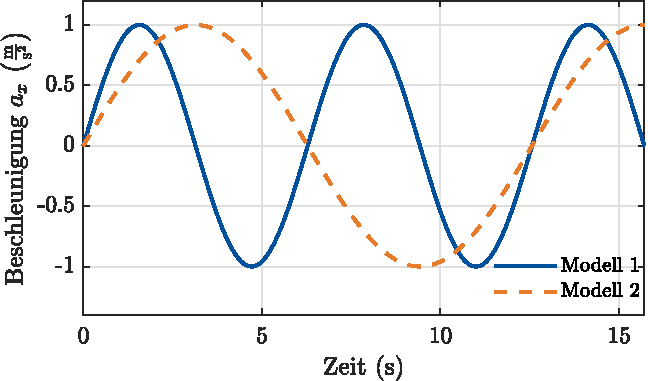
\includegraphics[]{template_einfach}
		\caption{Vergleich der zeitlichen Beschleunigungsverläufe der beiden Modellierungsansätze Hü (blau) und Hott (orange gestrichelt)}
		\label{fig.Template}
	\end{center}
\end{figure}

%%%%%%%%%%%%%%%%%%%%%%%%%%%%%%%%%%%%%%%%%%%%%%%%%%%%%%%%%%%%%%%%%%%%%%%%%%%%%%%%%%%%

\section{Software}
\subsection{Matlab, Corel}
Für Matlab und Corel sind an der Uni Hannover kostenlose Campuslizenzen verfügbar. Anleitungen zum Bezug sind unter https://www.luis.uni-hannover.de/softwarekatalog.html zu finden. Für Corel existiert am imes ein Plugin zur Nutzung von LaTeX-Befehlen. Das Plugin und die zugehörige Anleitung sind im Vorlagenordner zu finden. Alternativ zu Corel kann auch die freie Software Inkscape genutzt werden (https://inkscape.org).

\subsection{LaTeX}
Vorschläge für TeX-Distributionen:
\begin{itemize}
	\item MiKTeX (Windows): https://miktex.org/
	\item TeXLive (allg.): http://www.tug.org/texlive/
\end{itemize}

Vorschläge für Texteditoren:
\begin{itemize}
	\item TeXnicCenter (Windows): http://www.texniccenter.org/
	\item TeXMaker (allg.): http://www.xm1math.net/texmaker/
\end{itemize}

%%%%%%%%%%%%%%%%%%%%%%%%%%%%%%%%%%%%%%%%%%%%%%%%%%%%%%%%%%%%%%%%%%%%%%%%%%%%%%%%%%%%

\section{Literaturverweise}
Beispiele für Literaturverweise sind im Literaturverzeichnis zu finden, z.\,B. Journalbeitrag \cite{Ber59}, Konferenzbeitrag \cite{Hussong08}, Buch \cite{Wintermantel09}. Sofern nicht explizit anders eingestellt, taucht nur diejenige Literatur im Verzeichnis auf, auf die in der Arbeit verwiesen wird.

%%%%%%%%%%%%%%%%%%%%%%%%%%%%%%%%%%%%%%%%%%%%%%%%%%%%%%%%%%%%%%%%%%%%%%%%%%%%%%%%%%%%

\section{Eigene Befehle in LaTeX}
In LateX können auch eigene Befehle definiert und genutzt werden, \zB zur Verwendung immer wiederkehrender Formelzeichen. So kann beispielsweise ein Koordinatensystem $\ks{A}$ direkt mit dem Befehl \textbackslash ks\{A\} eingefügt werden. Eine Liste der Befehle ist in der Datei befehle.sty zu finden.

